
Экспремент 1.

На рисунке 5 представлены графики изменения $a(x)$ и $b(x)$, в зависимости от $x$, на рисунке 6 ряд распределения вероятностей количества заявок на орбите для следующих параметров системы $N=2$, $r_{0}=0,7, r_{1}=0,2, r_{2}=0,1, \lambda=0,8, \mu_{1}=0,6, \mu_{2}=1,5, q=0,25.$

\begin{figure}[H]
	\centering
	\begin{minipage}[h]{0.49\linewidth}
		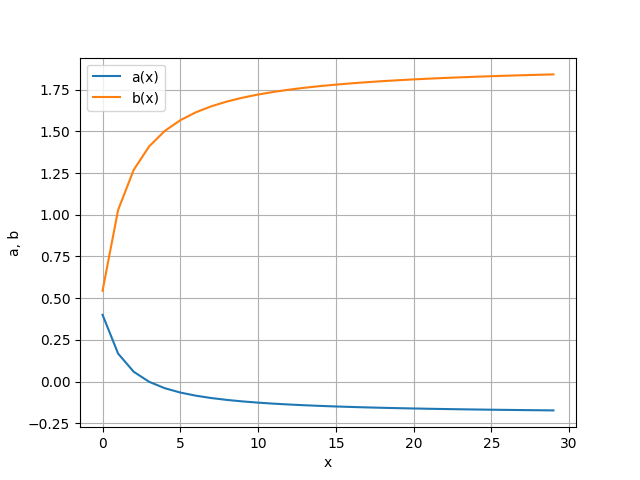
\includegraphics[width=0.8\linewidth]{ab2} 	
		\caption{Коэффициенты переноса $a(x)$ и диффузии $b(x)$}
		\label{ris:experimoriginal}
	\end{minipage}
	\hfill
	\begin{minipage}[h]{0.49\linewidth}
		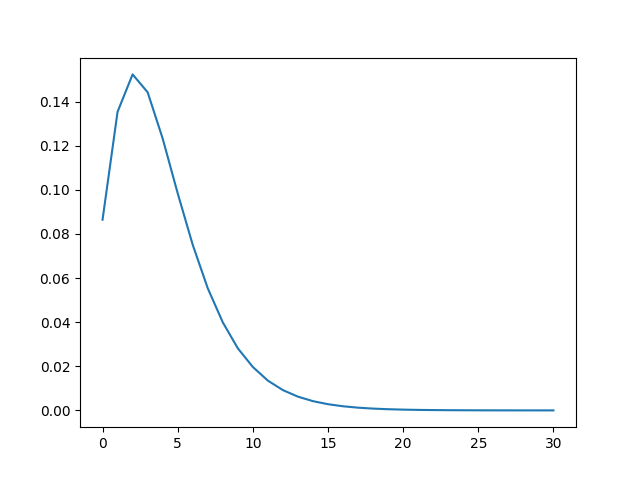
\includegraphics[width=0.8\linewidth]{P2} 
		\caption{Ряд распределения вероятностей числа заявок на орбите}
		\label{ris:experimcoded}
	\end{minipage}
\end{figure}
\noindent Экспремент 2.

На рисунке 7 представлены графики изменения $a(x)$ и $b(x)$, в зависимости от $x$, на рисунке 8 ряд распределения вероятностей количества заявок на орбите для следующих параметров системы $N=10$, $r_{0}=0,7, r_{1}=0,2, r_{2}=0,1, \lambda=0,8, \mu_{1}=0,6, \mu_{2}=1,5, q=0,25.$
\begin{figure}[H]
	\centering
	\begin{minipage}[h]{0.49\linewidth}
		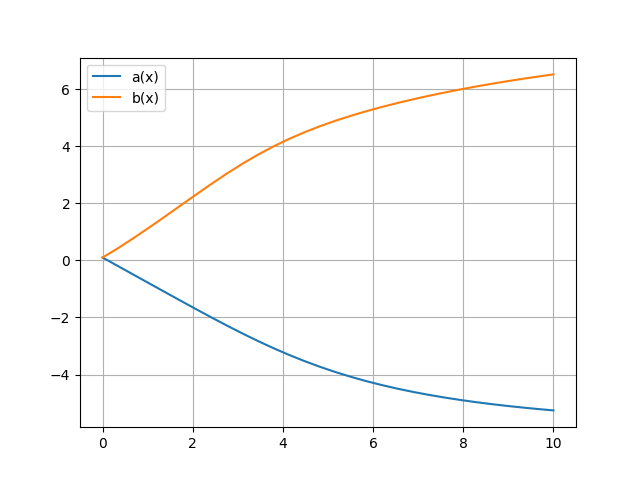
\includegraphics[width=0.8\linewidth]{ab10} 	
		\caption{Коэффициенты переноса $a(x)$ и диффузии $b(x)$}
		\label{ris:experimoriginal}
	\end{minipage}
	\hfill
	\begin{minipage}[h]{0.49\linewidth}
		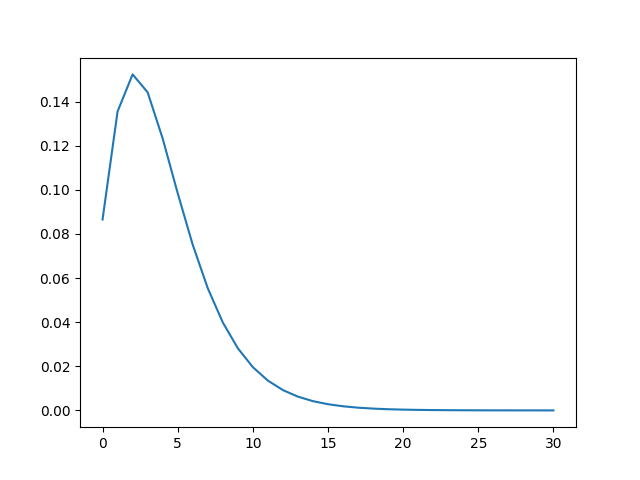
\includegraphics[width=0.8\linewidth]{P10} 
		\caption{Ряд распределения вероятностей числа заявок на орбите}
		\label{ris:experimcoded}
	\end{minipage}
\end{figure}

Численные результаты были получены с помощью библиотек NymPy [19] (для $a(x)$ и $b(x)$) и SimPy [15] языка Python.
Данные графики были построены с помощью библиотеки Mathplotlib [20] языка Python.